\label{sec:unified-experiments}

All experiments in this section use the clamped-free beam, static-field
eigenvectors, complete magnetic cosine, and SI parameters defined above.
The two-mode learning problem and its higher-order validation models therefore
share the same mechanics. The reference energy is
\begin{equation}
 \begin{aligned}
 h_\star(X,Y)&=\frac12\sum_{j=1}^2\nu_j(X_j^2+Y_j^2)+g(d^TX),\\
 g(s)&=1-\cos s-\frac12s^2 .
 \end{aligned}
 \label{eq:unified-reference-energy}
\end{equation}
Here $\nu=(1,6.152117504)$ and
$d=(0.225670773,0.321798806)^T$; one dimensionless energy unit is
$6.0\times10^{-7}$ J and $\tau=11.417287283t$.
The tip displacement in metres is
$0.013506054X_1+0.005470926X_2$.
These mappings are used for every reported displacement, slope, and energy
error, including the independent COMSOL comparison.

\subsection{Finite-feature identification and matched controls}
\label{sec:unified-learning-protocol}
The CHNN uses $z_j=(X_j+\mathrm{i}Y_j)/\sqrt2$, conjugate polynomial
features, and a complex exponential feature for the full cosine.
Its real energy readout is
\begin{equation}
 h_\vartheta=h_2+a\,g(d^TX)+m_4(X,Y)^TUc,
 \label{eq:unified-feature-readout}
\end{equation}
where $m_4$ lists the 35 degree-four real monomials in $(X_1,X_2,Y_1,Y_2)$.
If $v_4$ is the coefficient vector of $-(d^TX)^4/24$, the 34 columns of
$U$ span its orthogonal complement. The feature $g/\|v_4\|_2$ and
these complementary quartics give 35 fitted real parameters, avoid
duplicating the leading cosine term, and retain the complete analytic
cosine tail. The target corresponds to $a=1,c=0$ and is therefore in the
feature class. The stored matrix $U$, rather than idealized exact
orthogonality, is used in the certificate computations.

We compare real (R) and complex (C) implementations, each with either the
fixed mechanical quadratic part (G) or a fitted general quadratic part (B).
Thus GR and GC have 35 fitted real parameters, whereas BR and BC have 45.
The two representations span the same real energy class, receive identical
data, and use the same regularizer expressed in common real feature coordinates.
Both implementations evaluate their respective real or complex features.
Because the representations are related by an invertible transformation,
this comparison tests their numerical implementation within a common
hypothesis class.

For each seed in $\{17,43,91\}$, we generate 12 conservative trajectories
of 4 s from the two-mode Python Galerkin model, sampled at 129 times.
Initial modal radii are drawn uniformly from
$[0.03,0.20]$ and $[0.03,0.16]$, with independent uniform phases.
The largest training tip slope is $0.0891$ rad.
Each component of the dimensionless vector-field label receives independent
uniform noise in $[-10^{-6},10^{-6}]$; states are noiseless.
Linear readout fitting minimizes derivative mean-square error with a
$10^{-14}$ quadratic regularizer.
Eight independent trajectories, generated with a separate seed and
integrated for 16 s at 1601 output times, are held out in full.
The reference solver is DOP853 with relative and absolute tolerances
$2\times10^{-10}$ and $2\times10^{-12}$.
Tightening both tolerances by a factor of 100 changes the tip of the first
held-out trajectory by at most $1.92\times10^{-8}$ mm.

\begin{table*}[t]
\centering
\caption{Conservative held-out errors, mean $\pm$ sample standard deviation
over three training seeds. Each seed is evaluated on all eight independent
16 s trajectories. These are errors within the declared simulated model.}
\label{tab:unified-learning}
\small
\begin{tabular}{lccc}
\hline
Model & Tip RMSE (mm) & Slope RMSE (mrad) & Energy RMSE (nJ)\\
\hline
BR & $(2.28\!\pm\!0.75)10^{-5}$ & $(5.80\!\pm\!1.20)10^{-4}$ & $(3.21\!\pm\!0.51)10^{-6}$\\
BC & $(2.28\!\pm\!0.75)10^{-5}$ & $(5.80\!\pm\!1.20)10^{-4}$ & $(3.21\!\pm\!0.51)10^{-6}$\\
GR & $(1.20\!\pm\!0.71)10^{-5}$ & $(3.90\!\pm\!1.63)10^{-4}$ & $(3.14\!\pm\!0.71)10^{-6}$\\
GC & $(1.20\!\pm\!0.71)10^{-5}$ & $(3.90\!\pm\!1.63)10^{-4}$ & $(3.14\!\pm\!0.71)10^{-6}$\\
\hline
\end{tabular}
\end{table*}

Table~\ref{tab:unified-learning} and Fig.~\ref{fig:unified-learning}
show the benefit of fixing the known quadratic mechanics in this
experiment, while matched real and complex fits agree to numerical
precision. GC identifies $a=1.00326\pm0.00154$ with nonzero training
residuals. The energy error evaluates the true energy along the predicted
and reference states; it is not an energy-conservation surrogate for
trajectory accuracy. The small fitting errors reflect exact representation,
accurate synthetic derivatives, and deliberately controlled label noise.
They do not establish corresponding physical measurement accuracy.

\begin{figure*}[t]
\centering
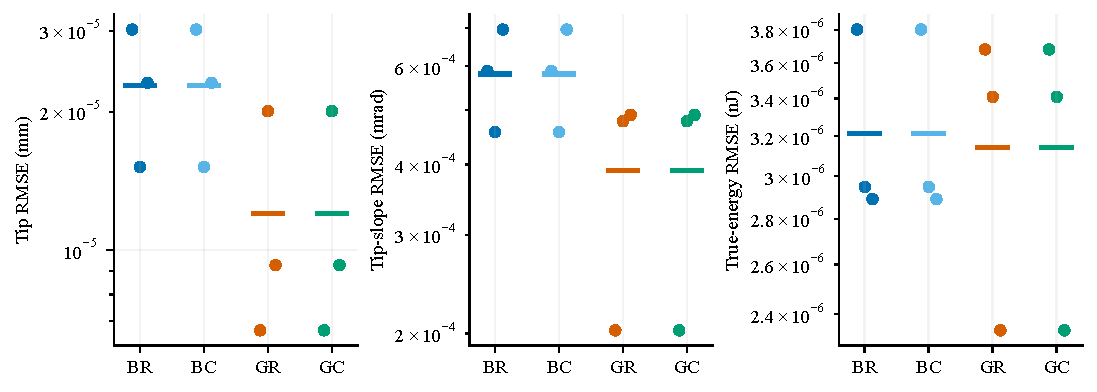
\includegraphics[width=\textwidth]{figures/fig_unified_learning.pdf}
\caption{Identical full-cosine beam data and real parameter budgets for the
four learning controls. Points are individual seeds and horizontal marks
are means. The quadratic mechanics prior changes the result; the matched
real/complex representation changes it only at numerical precision.}
\label{fig:unified-learning}
\end{figure*}

We also continue one independent initial condition for 200 s, or
363 first-mode linear periods, using the three primary GC fits.
The seed-level tip RMSE ranges from $1.38\times10^{-4}$ to
$4.03\times10^{-4}$ mm; the largest modal phase error is
$4.19\times10^{-4}$ rad. The relative drift of each learned model's own
energy remains below $5.11\times10^{-9}$ with conservative integration
at relative and absolute tolerances $2\times10^{-11}$ and $2\times10^{-13}$.
Figure~\ref{fig:unified-long} shows its Poincar\'e section, phase error,
and numerical energy drift. These finite-time diagnostics assess the
fitted dynamics; they do not estimate the measure of KAM tori or replace
the analytic certificate.

\begin{figure*}[t]
\centering
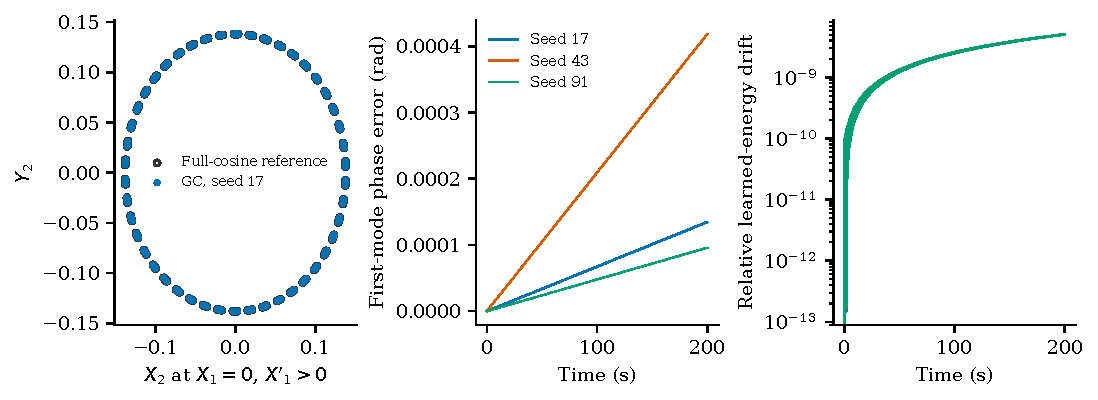
\includegraphics[width=\textwidth]{figures/fig_conservative_long_horizon.pdf}
\caption{Conservative 200 s continuation of an independent initial state.
Left: 364 upward crossings of $X_1=0$ for the reference and GC17.
Middle: unwrapped first-mode phase errors of the three learned energies.
Right: each learned energy's relative integration drift. All ports are
closed for these conservative diagnostics.}
\label{fig:unified-long}
\end{figure*}

\subsection{A nonzero-loss certificate for the fitted magnetic energy}
\label{sec:unified-loss-certificate}
The feature derivatives make the empirical Gram matrix and the complete
quartic Taylor map computable. We repeat the same three fits at noise
amplitudes $10^{-8}$ and $10^{-9}$, in addition to the $10^{-6}$
experiments. Outward-rounded interval calculations enclose the derivatives
of the analytic sine feature at the stored states, the Gram inverse
residual, the observed loss, clean-label rounding, and the conversion from
readout weights to the exported energy coefficients.
The degree-17 sine series is enclosed with its degree-19 remainder.

For the target magnetic quartic,
$A_{jj}=-d_j^4/8$ and $A_{12}=-d_1^2d_2^2/4$.
This twist is indefinite and nonsingular. Exact rational arithmetic on the
stored dyadic $d$ gives the conservative lower bound
$\sigma_{\min}(A_\star)>3.03081\times10^{-4}$.
If $G$ is the derivative Gram matrix, $B$ the quartic coefficient map,
$\ell$ the noisy derivative MSE, and $\eta_{\rm eff}$ the enclosed noise
and arithmetic budget, the verified sufficient inequality is
\begin{equation}
 \sqrt{19}\left(
 \|B\|_2\frac{\sqrt{\ell}+\eta_{\rm eff}}
                  {\sqrt{\lambda_{\min}(G)}}+\delta_{\rm dec}
 \right)<\sigma_{\min}(A_\star),
 \label{eq:unified-verified-twist}
\end{equation}
where $\delta_{\rm dec}$ encloses readout decoding roundoff.
At $\eta=10^{-8}$, Table~\ref{tab:unified-gram} verifies this inequality
with strictly positive losses for all seeds. Thus the data-dependent
error bound itself transfers nondegeneracy to the actual learned
Hamiltonians. The local KAM conclusions additionally use the nonresonance
and analytic normal-form hypotheses proved for this same model.
This table alone does not certify a finite experimental oscillation radius.
For the primary $10^{-6}$ fits, this sufficient error bound is too loose;
their directly computed twist singular values are nevertheless between
$5.78\times10^{-4}$ and $5.93\times10^{-4}$.

\begin{table*}[t]
\centering
\caption{Enclosed loss-to-twist checks at noise amplitude $10^{-8}$.
All twist-error upper bounds are below $3.03081\times10^{-4}$.}
\label{tab:unified-gram}
\small
\begin{tabular}{rccc}
\hline
Seed & Noisy MSE & Gram eigenvalue lower bound & Twist-error upper bound\\
\hline
17 & $3.387\times10^{-17}$ & $6.0167\times10^{-8}$ & $2.8112\times10^{-4}$\\
43 & $3.275\times10^{-17}$ & $2.2734\times10^{-7}$ & $1.4374\times10^{-4}$\\
91 & $3.283\times10^{-17}$ & $2.0968\times10^{-7}$ & $1.4973\times10^{-4}$\\
\hline
\end{tabular}
\end{table*}

\subsection{Learning dissipation and opening the magnetic input port}
The imaginary readout is the nonnegative Rayleigh potential
$\mathcal D_\gamma(v)=\gamma\sum_jv_j^2/(2\nu_j)$, with $v=h_{\vartheta,Y}$.
For each seed, eight additional damped, unforced 5 s trajectories provide
noisy derivative labels. Nonnegative least squares fits the single
$\gamma$ using the already fitted conservative gradient. In particular,
the decoder retains the learned momentum-dependent quartics:
\begin{equation}
 \begin{aligned}
 X'&=h_{\vartheta,Y},\\
 Y'&=-h_{\vartheta,X}-\gamma\operatorname{diag}(\nu^{-1})h_{\vartheta,Y}\\
   &\quad+u\,d\cos(d^TX).
 \end{aligned}
 \label{eq:unified-learned-port}
\end{equation}
The fitted dimensional mass-drag coefficients are
$0.555585710$, $0.555587102$, and $0.555584024$ s$^{-1}$, compared with
$0.555585237$ s$^{-1}$ for the generator.
On six independent driven trajectories with amplitudes 4--8 mT and
frequency ratios $0.65$--$1.20$ relative to the biased first frequency,
the three seed-level tip RMSEs are
$8.83\times10^{-5}$, $1.37\times10^{-4}$, and
$6.40\times10^{-5}$ mm. Closing the learned drag port increases the
tip RMSE to approximately $3.01$ mm.
The integrated work balance is
\begin{equation}
 \begin{aligned}
 h_\vartheta(\tau)-h_\vartheta(0)
 &=\int_0^\tau u\cos(d^TX)d^Th_{\vartheta,Y}\,ds\\
 &\quad-\int_0^\tau\gamma\sum_jh_{\vartheta,Y_j}^2/\nu_j\,ds.
 \end{aligned}
\end{equation}
Its largest numerical residual across these cases is
$4.41\times10^{-17}$ J.
These driven tests assess the port model, rather than autonomous KAM
persistence. Some stress cases exceed the channel clearance and are
free-motion continuations; safe operating trajectories are evaluated
separately with the physical energy bound and input governor.

\begin{figure*}[t]
\centering
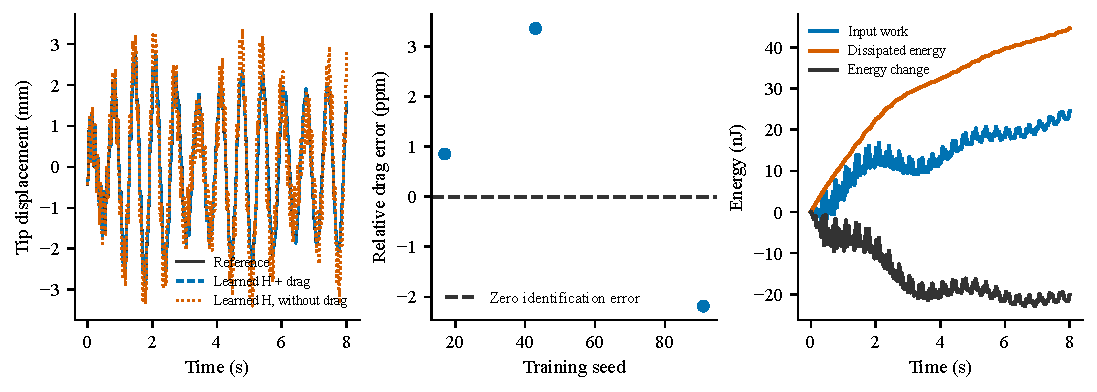
\includegraphics[width=\textwidth]{figures/fig_unified_ports.pdf}
\caption{The same learned conservative energy with an identified
nonnegative drag readout and magnetic input port. Left: an independent
driven trajectory and the drag ablation. Middle: signed relative errors
in the drag coefficient. Right: supplied work, dissipated energy, and
stored-energy change for that trajectory.}
\label{fig:unified-ports}
\end{figure*}

\subsection{Independent COMSOL assembly and nonlinear time integration}
\label{sec:unified-comsol}
COMSOL Multiphysics 6.3 independently assembles the same 32-element
clamped-free beam and solves its nonlinear magnetic-tip response.
The relative Frobenius differences between the exported and Python
consistent-mass matrices are $7.75\times10^{-15}$ for mass and
$3.05\times10^{-14}$ for bending stiffness.
The nonlinear held-out COMSOL trajectory starts from rest, uses the
same mass drag, and applies
\begin{equation}
 B_y(t)=0.006\,[1-\exp(-(t/0.25)^2)]\sin(\Omega t)\quad\mathrm{T}
\end{equation}
with $\Omega=9.4449490256$ rad/s for 8 s, relative tolerance $10^{-7}$,
and 2001 output samples.
The exported nodal displacement, rotation, velocity, and angular velocity
are evaluated directly, with no fitting to this driven trajectory.
Its peak tip displacement is $3.09032$ mm.
A separate COMSOL solve with relative tolerance $10^{-8}$ changes the
tip by $4.59\times10^{-5}$ mm RMSE and reduces its discrepancy against
the full Python FE solution to $1.03\times10^{-5}$ mm RMSE. The original
held-out dataset is used for the primary comparison below.

\begin{table*}[t]
\centering
\caption{Independent nonlinear COMSOL trajectory comparison. Modal models
use the common static-field chart. GC includes learned drag; its range
covers the three primary training seeds.}
\label{tab:unified-comsol}
\small
\begin{tabular}{lcc}
\hline
Predictor & Tip RMSE (mm) & Maximum tip error (mm)\\
\hline
2-mode exact cosine & $0.0156168$ & $0.0226548$\\
4-mode exact cosine & $0.00407422$ & $0.00592596$\\
8-mode exact cosine & $0.00102484$ & $0.00152782$\\
64-mode Python FE & $0.00005614$ & $0.00011835$\\
2-mode learned GC & $0.0156171$--$0.0156177$ & $0.0226545$--$0.0226549$\\
\hline
\end{tabular}
\end{table*}

The nested modal comparison in Table~\ref{tab:unified-comsol} separates
reduction error from learning error. Against the exact two-mode response,
GC contributes only $1.81\times10^{-6}$--$3.48\times10^{-6}$ mm tip RMSE
for this input. Against COMSOL, both have approximately $0.0156$ mm RMSE.
The two-mode maximum slope discrepancy is $3.69$ mrad; its true stored-energy
RMSE is $0.132$ nJ. These discrepancies decrease with modal enrichment.
Figure~\ref{fig:unified-comsol} shows the response and both error scales.
The primary training data were generated by the two-mode Python
Galerkin model; the COMSOL time history is an independent held-out
validation dataset. Neither dataset is a physical hardware measurement.

\begin{figure*}[t]
\centering
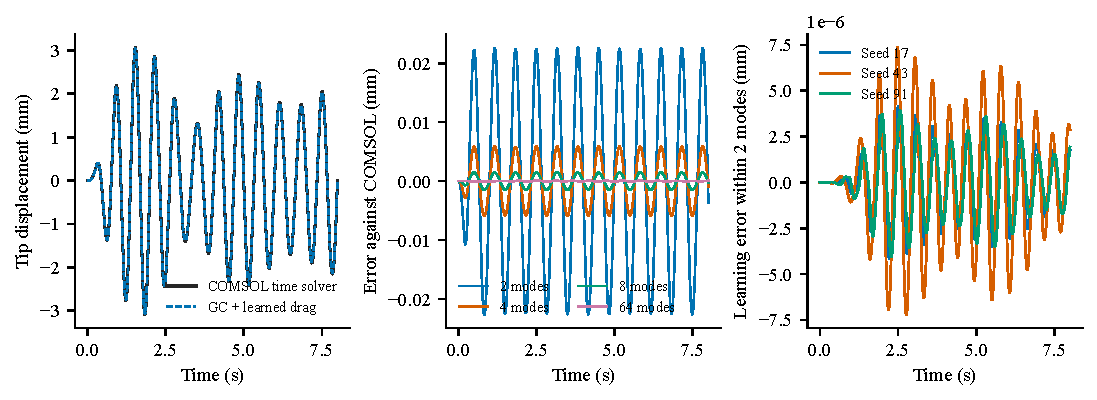
\includegraphics[width=\textwidth]{figures/fig_comsol_heldout.pdf}
\caption{Independent nonlinear COMSOL time integration. Left: COMSOL and
the learned two-mode GC response with learned drag. Middle: errors of
the nested exact-cosine modal models against COMSOL. Right: the additional
GC identification error within the two-mode model. Reduction error is
the larger contribution in this validation.}
\label{fig:unified-comsol}
\end{figure*}

\subsection{COMSOL-derived training data and an independent integral check}
\label{sec:comsol-identification}
We generate a separate conservative COMSOL dataset comprising four 4 s
training trajectories and two independent 8 s test trajectories, sampled
every 0.004 s. Initial displacements and velocities excite both retained
modes. The remaining 62 modes receive the static response to the nonlinear
magnetic residual and its compatible first time derivative; all 64 modes
remain active during integration. This initial tail condensation is not
assumed to be an exact nonlinear invariant manifold. Native solver-vector
checks confirm that the exported initial displacement and velocity are
correct; small changes introduced by consistent initialization are handled
by starting each predictor from the actual exported state.

The derivative-label construction requires care. At the stored output
times, the exported second time derivatives differentiate a time
interpolant and show a substantial lag relative to the velocity evolution.
For example, the first trajectory has a dimensionless modal equation-residual
RMS of $4.58\times10^{-2}$ when those derivatives are used directly.
We therefore reconstruct instantaneous acceleration from the exported
COMSOL mass and stiffness matrices:
\begin{equation}
 \ddot q=M_{\rm C}^{-1}
 \left[-K_{\rm C}q-\mu B_0\sin(\theta_{\rm tip})e_\theta\right].
 \label{eq:comsol-force-labels}
\end{equation}
The training states and velocities therefore come from the COMSOL
time solver, while the acceleration labels use known physical force
balance. This is surrogate identification for the declared mechanical
model with force-balance labels. The unresolved-mode force is included:
its largest component is $3.36\times10^{-9}$ in dimensionless
units for the checked training trajectory, and the remaining reconstructed
equation-residual RMS is $1.81\times10^{-10}$.

These COMSOL-based models are fitted separately from the primary
Python-trained GC models. Three seeds vary the
additional componentwise label noise, bounded by $10^{-6}$, while using
the same four COMSOL trajectories. The real/complex and prior/no-prior
controls use the same parameter budgets as before.

An independent check uses only the COMSOL displacement and velocity
samples. A nine-point closed Newton--Cotes rule integrates the vector-field
features on nonoverlapping 0.032 s windows, and the observed state
increments provide the regression targets. No acceleration or
force-balance label enters this integral fit.
With the initial solver settings (relative tolerance $10^{-6}$ and
scaled absolute tolerance $10^{-5}$), the integral residual is too large
to resolve the weak magnetic correction reliably: on the first trajectory,
its RMS is 2.16 times the nonlinear magnetic signal. An unconstrained
35-feature integral fit then yields $a=1.437$, illustrating that a good
fit to a numerically dispersed trajectory need not recover the physical
magnetic coefficient. A stricter COMSOL solve, with relative tolerance
$10^{-8}$ and scaled absolute tolerance $10^{-7}$, reduces that ratio
to 0.112 on the same trajectory. This independent data-quality check
resolves time-integration error that the force-balance loss alone
does not detect.

All six trajectories were then integrated with these stricter
tolerances. The refined runs use
generalized-alpha integration with high-frequency spectral radius zero
and backward-Euler consistent initialization. The four refined training
trajectories provide 500 integral windows, or 2000 scalar equations, for
the 35 real readout parameters. The resulting GC model has
$a=1.0223248822$ and a nonzero averaged-derivative integral RMS residual
of $4.0524\times10^{-7}$. The corresponding residuals of the quadratic
prior alone and the physical full-cosine target are
$3.9099\times10^{-6}$ and $6.6454\times10^{-7}$; the nonlinear magnetic
signal RMS is $3.6601\times10^{-6}$.
The fitted quartic twist has minimum singular value
$5.1166\times10^{-4}$. The conservative weights were frozen before
evaluating the two independent refined test trajectories.

\begin{table*}[t]
\centering
\caption{Independent refined COMSOL tests of the GC model identified
only from displacement and velocity increments. Predictions start from
each actual exported initial state. Energy errors use the physical
stored-energy function evaluated along the learned trajectory.}
\label{tab:comsol-integral-tests}
\small
\begin{tabular}{lccccc}
\hline
Test & Tip RMSE & Max. tip error & Slope RMSE & Energy RMSE & Exact 2-mode\\
 & ($\mu$m) & ($\mu$m) & (mrad) & (nJ) & tip RMSE ($\mu$m)\\
\hline
1 & $0.14836$ & $0.39240$ & $0.008677$ & $0.0002067$ & $0.24172$\\
2 & $0.05140$ & $0.17435$ & $0.002411$ & $0.0002253$ & $0.27459$\\
\hline
\end{tabular}
\end{table*}

Table~\ref{tab:comsol-integral-tests} and
Figure~\ref{fig:comsol-integral-tests} report the held-out errors.
The integral fit partly absorbs the remaining time-solver dispersion:
its agreement with COMSOL is better than that of the exact closed
two-mode target, despite a $2.23\%$ error in the cosine multiplier.
These errors quantify identification against simulated observations.
The requested solver tolerances do not supply a rigorous defect budget
for applying the loss-based certificate to these integral residuals.
The separate two-mode short-trajectory experiment in
Section~\ref{sec:validated-integral-learning} supplies a verified integral
defect budget and the corresponding loss-based certificate for its own
frozen fitted function.

\begin{figure*}[t]
\centering
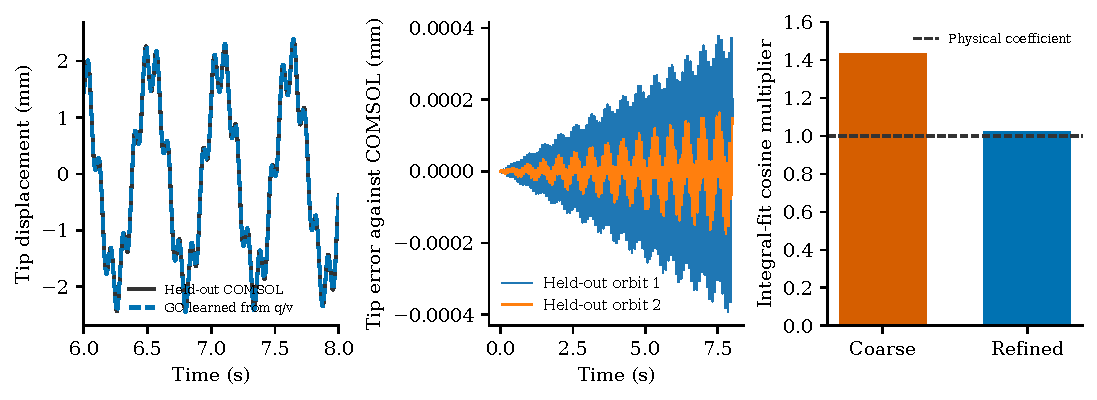
\includegraphics[width=\textwidth]{figures/fig_comsol_qv_identification_refined.pdf}
\caption{Identification using full-FE COMSOL displacement and velocity
outputs only. Left: independent test response. Middle: prediction errors
for both held-out trajectories. Right: the fitted cosine multiplier
under the two declared COMSOL tolerance settings; the physical value is
one. The refined coefficients are held fixed during the subsequent evaluations.}
\label{fig:comsol-integral-tests}
\end{figure*}

For comparison, the separately fitted models using the known-force
labels in~\eqref{eq:comsol-force-labels} recover $a=1.0000690$ without
added label noise. With the three added-noise seeds, the prior-informed
GC models give $0.25347$--$0.25940\,\mu$m pooled tip RMSE against the
same refined COMSOL tests; their additional error relative to the
closed two-mode trajectories is $0.00364$--$0.00771\,\mu$m.
Matched real and complex features again give coincident results to
numerical precision.

Finally, the position--velocity fit is used in the
independent a posteriori proof of
Section~\ref{sec:unified-aposteriori}. Its complete cosine and all fitted
quartic coefficients yield an analytic residual below
$2.7330\times10^{-77}$ and a theorem smallness quantity below $0.031746$.
The resulting exact invariant torus has a tip-displacement witness above
$1.8977374$ mm and a whole-centreline upper bound below $1.8977433$ mm.
This certificate concerns the actual fitted Hamiltonian and does not
require its coefficients to equal the physical target.
The same frozen conservative readout is paired with a nonnegative
drag coefficient refitted on the existing Python damped-beam trajectories,
$\gamma=0.0486617702$ for seed 17. Its independent driven COMSOL tip
RMSE is $0.015622$ mm. Section~\ref{sec:unifiedlearnedcontrol} then uses
this same energy, full gradient and Hessian, and drag readout to generate
the magnetic tracking input.
